\documentclass{ieeeaccess}
\usepackage{cite}
\usepackage{amsmath,amssymb,amsfonts}
\usepackage{algorithmic}
\usepackage{graphicx}
\usepackage{caption}
\usepackage{subcaption}
\usepackage{textcomp}
\usepackage{cite}
\usepackage{tabularx}
\usepackage{dblfloatfix}
\usepackage{float}
\usepackage{multirow}
\usepackage{booktabs}
\usepackage{hyperref}
\hypersetup{
    colorlinks=true,
    linkcolor=blue,
    citecolor=blue,
    filecolor=black,
    urlcolor=blue
}

\def\BibTeX{{\rm B\kern-.05em{\sc i\kern-.025em b}\kern-.08em
    T\kern-.1667em\lower.7ex\hbox{E}\kern-.125emX}}
\begin{document}
\history{}
\doi{}

\title{Machine Learning-Based Classification of Abnormal Gait Patterns Using Wearable Gyroscope Data}

\author{
\uppercase{Stamatios Orfanos\authorrefmark{1}~\href{https://orcid.org/0009-0005-5042-9408}{
\includegraphics[height=0.6ex]{orcid_logo.png}}},
\uppercase{Thanita Sanghan\authorrefmark{2}~\href{https://orcid.org/0009-0005-1693-5673}{
\includegraphics[height=0.6ex]{orcid_logo.png}}},
\uppercase{Andreas Menychtas\authorrefmark{3}~\href{https://orcid.org/0000-0002-4510-5522}{
\includegraphics[height=0.6ex]{orcid_logo.png}}},
\uppercase{Christos Panagopoulos\authorrefmark{1}~\href{https://orcid.org/}{
\includegraphics[height=0.6ex]{orcid_logo.png}}},
\uppercase{Ilias Maglogiannis\authorrefmark{3}~\href{https://orcid.org/0000-0003-2860-399X}{
\includegraphics[height=0.6ex]{orcid_logo.png}}},
\uppercase{Surapong Chatpun\authorrefmark{2}~\href{https://orcid.org/0000-0002-6888-5170}{
\includegraphics[height=0.6ex]{orcid_logo.png}}}
}

\address[1]{BioΑssist SA, Kastritsiou 4, Rio 265 04, Greece}
\address[2]{Department of Biomedical Sciences and Biomedical Engineering, Faculty of Medicine, Prince of Songkla University, Songkhla 90110, Thailand}
\address[3]{University of Piraeus, Department of Digital Systems, 80 Karaoli \& Dimitriou Str., 18534 Piraeus, Greece}


\tfootnote{This work was supported in part by the Faculty of Medicine, Prince of Songkla University, Thailand, under
Grant 64-386-25-2; and in part by the Horizon Europe Framework Program under Grant 101086348.
}

\corresp{Corresponding author: Surapong Chatpun (e-mail: surapong.c@psu.ac.th).}

\begin{abstract}
Accurate detection of gait abnormalities is an important prerequisite for clinical screening and rehabilitation monitoring in stroke populations. In this study, 
we present a lightweight machine learning framework for binary classification of normal versus abnormal gait using statistical features derived from wearable 
gyroscope sensors. Specifically, we extract extremal statistical features from the z-axis angular velocity of both shanks and evaluate multiple classifiers, 
including logistic regression, support vector machines, and ensemble methods. A leave-one-out cross-validation (LOOCV) strategy is employed to maximize 
subject-level generalization under limited data conditions. Experimental results demonstrate that several models achieve accuracy and area under the curve (AUC) 
values exceeding 0.95, with ensemble-based classifiers exhibiting particularly robust performance. These findings highlight the potential of minimal yet biomechanically 
meaningful gyroscope features for screening-level gait abnormality detection in wearable and remote monitoring scenarios. The proposed pipeline is computationally 
efficient and suitable for resource-constrained sensing environments, providing a foundation for future extensions toward severity-aware analysis and real-time 
rehabilitation support.
\end{abstract}


\begin{keywords}
Gait classification, Gyroscope features, Machine learning, Stroke Rehabilitation, Wearable sensors
\end{keywords}

\titlepgskip=-15pt

\maketitle
\section{Introduction}
\label{sec:introduction}
The study of human gait has long been recognized as a fundamental method for assessing motor function, neurological health, and musculoskeletal integrity. 
Gait analysis, defined as the systematic study of human locomotionn as it offers critical insights into motor control, functional ability, and the presence of 
pathological deviations \cite{ref1, ref2}. While observational assessments are commonly used in clinical practice, they often lack the precision required 
to detect and quantify subtle gait asymmetries without dedicated instrumentation. Traditional gait analysis systems, typically found in motion analysis 
laboratories, utilize advanced tools such as optical motion capture, force platforms, and surface electromyography to capture high-resolution biomechanical 
data \cite{ref3}. Despite their accuracy, these systems are characterized by high financial costs, space requirements, and complex operational demands, with 
total investments frequently reaching several million dollars \cite{ref4}.

This economic and logistical barrier becomes particularly problematic in the context of stroke rehabilitation, where timely, repeated 
assessments of motor asymmetry are vital. Stroke survivors often experience hemiparesis, a condition that leads to asymmetrical gait 
characterized by unequal stance or swing phases between limbs \cite{ref5}. Detecting and quantifying such asymmetries in a reliable and scalable 
manner remains a major challenge in both inpatient and outpatient care settings. The early and continuous identification of gait deviations 
is vital for creating personalized rehabilitation programs, tracking recovery progress, and preventing secondary complications such as joint degeneration 
or in some cases falls \cite{ref6}, \cite{ref7}.

With recent advances in the Internet of Things (IoT) and embedded computing, there has been a surge of interest in using wearable sensors, 
particularly inertial measurement units (IMUs), to provide low-cost and scalable alternatives to lab-based gait analysis systems \cite{ref8}–\cite{ref10}. 
These sensors, such as accelerometers and gyroscopes, enable three-dimensional kinematic monitoring in every day environments, offering 
an ideal platform for remote monitoring and rehabilitation \cite{ref11}, \cite{ref12}. Combined with modern machine learning techniques, wearable 
IMU data can be processed to extract relevant temporal and kinematic features, enabling the classification of abnormal gait patterns with 
high accuracy \cite{ref13}, \cite{ref14}.

Previous studies have applied models such as Support Vector Machines (SVM), Random Forests, and Convolutional Neural Networks (CNN) to 
classify human movement patterns using IMU-derived features \cite{ref15}, \cite{ref16}. However, these approaches often rely on extensive datasets, high 
computational resources, or complicated feature extraction pipelines. Furthermore, there remains a lack of lightweight, interpretable methods specifically 
tailored to detect clinically meaningful gait asymmetries—especially in populations recovering from neurological events such as stroke.

To address this gap, this work proposes a minimal-feature, machine learning-based pipeline for classifying normal versus abnormal gait signals using 
statistical extrema from bilateral gyroscope signals. The approach is designed to be computationally efficient and interpretable, making it suitable 
for embedded deployment in wearable rehabilitation systems. A leave-one-out cross-validation (LOOCV) strategy is employed to ensure model 
generalizability across individuals, particularly relevant for heterogeneous stroke populations.

The contributions of this work are twofold:
\begin{itemize}
    \item the use of biomechanically relevant, low-dimensional gyroscope features for gait classification
    \item a comparative evaluation of classic machine learning models using LOOCV on subject-level data
\end{itemize}
 
 


\section{Related Work}
\label{sec:related_work}
The use of inertial measurement units (IMUs) for gait analysis has gained traction in both research and clinical domains, because of their  portability, affordability, 
and ability to collect kinematic data in real-world environments. There has been a number of studies that have validated the feasibility and accuracy of IMU-based 
gait monitoring in healthy, aging and impaired populations. An example of this case is the research by Yoon \textit{et al.} \cite{ref20}, where a cross-sectional 
study was conducted using wearable IMUs to assess gait parameters in younger and older adults, confirming their reliability compared to traditional 
magnetometer-based systems. Similarly, systematic reviews, like the one by Prisco \textit{et al.} \cite{ref21} and Zhu \textit{et al.} \cite{ref22} have 
comprehensively examined the validity of wearable inertial sensors, highlighting the effectiveness of single- and multi-point IMU configurations for capturing 
clinically relevant gait metrics.

Many studies have focused on gait event detection—such as identifying heel strikes or toe-offs—using IMUs. 
Voisard \textit{et al.} \cite{ref23} developed an automatic gait event detection algorithm capable of operating accurately across healthy 
individuals and patients with moderate to severe impairments, including those recovering from stroke. Larsen \textit{et al.} \cite{ref24} extended this line 
of research by introducing a neural network-based approach optimized for smartphone-embedded IMUs, achieving high detection accuracy in real-world conditions.

Despite the technical progress, much of the literature focuses on algorithmic sophistication or system validation rather than clinical interpretability or 
rehabilitation deployment. Bhole and Gokhale \cite{ref25} proposed an IMU-based system for basic gait event analysis, while Gudmundsson and 
Runarsson \cite{ref26} evaluated IMU sensor integration with heuristic rules for movement phase detection. However, these studies often lack the subject-specific 
generalization or low-complexity pipelines required for real-time, embedded medical use.

Notably, few works have been designed specifically for stroke rehabilitation, where gait asymmetry and inter-subject variability are prevalent. 
Patterson \textit{et al.} \cite{ref27} quantified temporal gait asymmetries among community-ambulating stroke survivors, while Zhao \textit{et al.} 
\cite{ref28} presented a dual foot-mounted IMU system for rehabilitation assessment in patients with cerebral thrombosis. Their system used an 
inequality-constrained ZUPT-aided inertial navigation approach to estimate gait parameters. However, these approaches often rely on dense feature sets 
or require manual tuning, making them less suitable for scalable deployment.

Although these previous studies have laid the groundwork for IMU-based gait analysis, there remains a lack of lightweight, interpretable, and clinically 
deployable methods tailored specifically for stroke-affected populations. This work addresses that gap by proposing a minimal-feature, high-performance 
classification pipeline using bilateral gyroscope extrema—optimized for subject-level generalization and embedded rehabilitation contexts.

\section{Materials and Methods}
\label{sec:materials_and_methods}

Building on the limitations highlighted in prior studies, this work introduces a simple yet effective classification framework for detecting abnormal gait patterns. 
The approach relies on just four carefully selected features derived from gyroscope signals—extremal values that are both biomechanically meaningful and easy to compute. 
Designed with practical deployment in mind, the framework prioritizes efficiency and interpretability, making it well-suited for use in wearable systems. To ensure that 
the model generalizes well across individuals, particularly in diverse clinical populations, we employ a leave-one-out cross-validation (LOOCV) strategy.

\subsection{Dataset Description}
The dataset used in this study was collected from a total of 18 participants, comprising 9 healthy individuals and 9 stroke survivors. 
The inclusion of both able-bodied and neurologically impaired subjects was intended to support the development of a binary classification 
model capable of distinguishing between normal and abnormal gait patterns. 

**At the time of writing, detailed demographic data (e.g., age, gender, affected limb) are being finalized and will be presented in a subsequent demographics table.

All participants underwent gait data collection using wearable inertial measurement units (IMUs). Each subject was equipped with sensors placed on the left and right 
shanks, as well as the left and right thighs as seen on . These positions were selected to capture comprehensive lower-limb kinematic data, with particular emphasis on the 
angular velocity along the z-axis—corresponding to the rotational movement of the legs during gait. The IMUs recorded tri-axial gyroscope data at a consistent 
sampling rate of 100Hz, and sessions were conducted under supervised walking trials on a flat indoor surface to ensure safety and signal consistency.

\begin{figure}[h]
    \centering
    \includegraphics[width=0.8\textwidth]{Images/.png}
    \caption{Placement of IMUs on the lower limbs during data collection.}
    \label{fig:imu_placement}
\end{figure}

\subsection{Feature Extraction}




\subsection{Classification Models}

\subsection{Evaluation Strategy}

\subsection{Dataset Description}

\section{Experimental Results}
\label{sec:experimental_resuts}
This section presents the classification performance of the various machine learning models using the selected gyroscope-based features. 

\subsection{Model Accuracy and AUC}
Starting with the Fig.~\ref{fig:accuracy_barplot}, the bar plot shows the classification accuracy of each model using the selected features: minimum and maximum 
values of the z-axis angular velocity from the left and right leg. The models tested include Logistic Regression, Random Forest, Support Vector Machines (SVM) 
with linear, polynomial, and RBF kernels, XGBoost, and K-Nearest Neighbors (KNN). 

\begin{figure}[h]
    \centering
    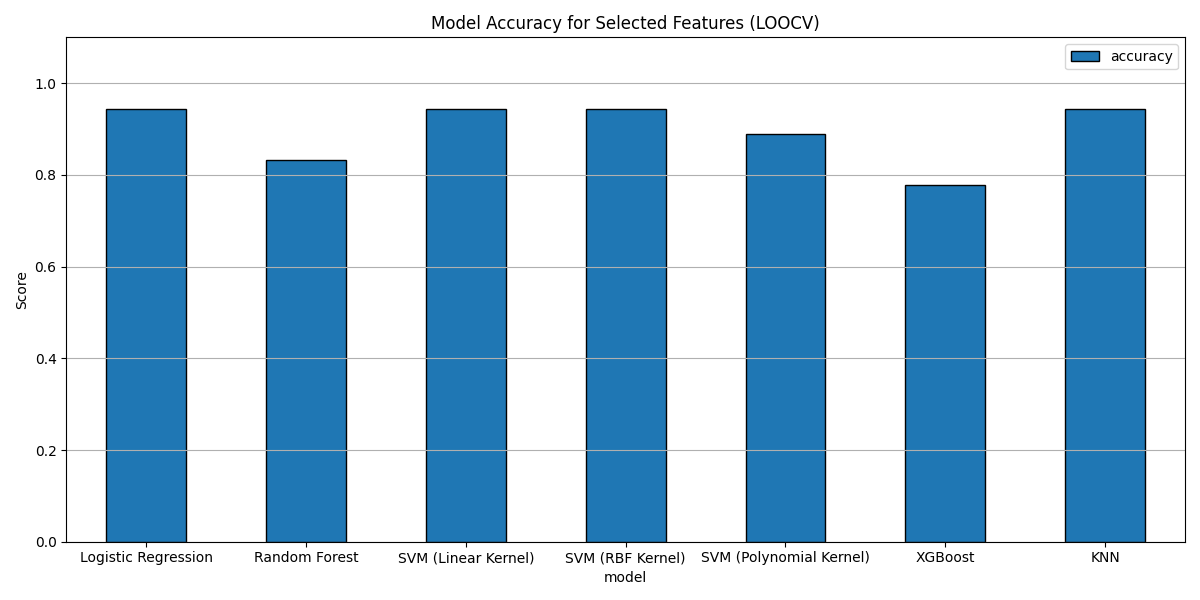
\includegraphics[width=0.5\textwidth]{Images/selected_features_accuracy.png}
    \caption{Barplot of Classification Accuracy for All Classifiers Using LOOCV}
    \label{fig:accuracy_barplot}
\end{figure}


The highest accuracy (94.44\%) was achieved by \textit{KNN}, \textit{Logistic Regression}, and \textit{SVM (Linear/RBF Kernel)}. In contrast, \textit{XGBoost} 
yielded the lowest accuracy (77.78\%). As shown in Table~\ref{tab:metrics}, these high-performing models also achieved an $AUC$ of $1.00$. 

\begin{table}[htbp]
    \caption{Accuracy and AUC for All Classifiers Using LOOCV}
    \label{tab:metrics}
    \centering
    \begin{tabular}{lcc}
    \toprule
    \textbf{Model} & \textbf{Accuracy} & \textbf{AUC} \\
    \midrule
    Logistic Regression     & 0.944 & 1.000 \\
    Random Forest           & 0.833 & 0.975 \\
    SVM (Linear Kernel)     & 0.944 & 1.000 \\
    SVM (RBF Kernel)        & 0.944 & 1.000 \\
    SVM (Polynomial Kernel) & 0.889 & 0.951 \\
    XGBoost                 & 0.778 & 0.605 \\
    KNN                     & 0.944 & 1.000 \\
    \bottomrule
    \end{tabular}
\end{table}

\newpage
\subsection{ROC Curve Analysis}
Fig.~\ref{fig:roc_curves} presents the ROC curves for all classifiers. \textit{KNN}, \textit{SVM (RBF/Linear)}, and \textit{Logistic Regression} show 
perfect discrimination with an AUC of 1.00. The \textit{Random Forest} model closely follows with an AUC of 0.975. The underperformance of \textit{XGBoost} 
is clearly visible with a notably flatter curve, suggesting difficulties in threshold-based separation.

\begin{figure}[h]
    \centering
    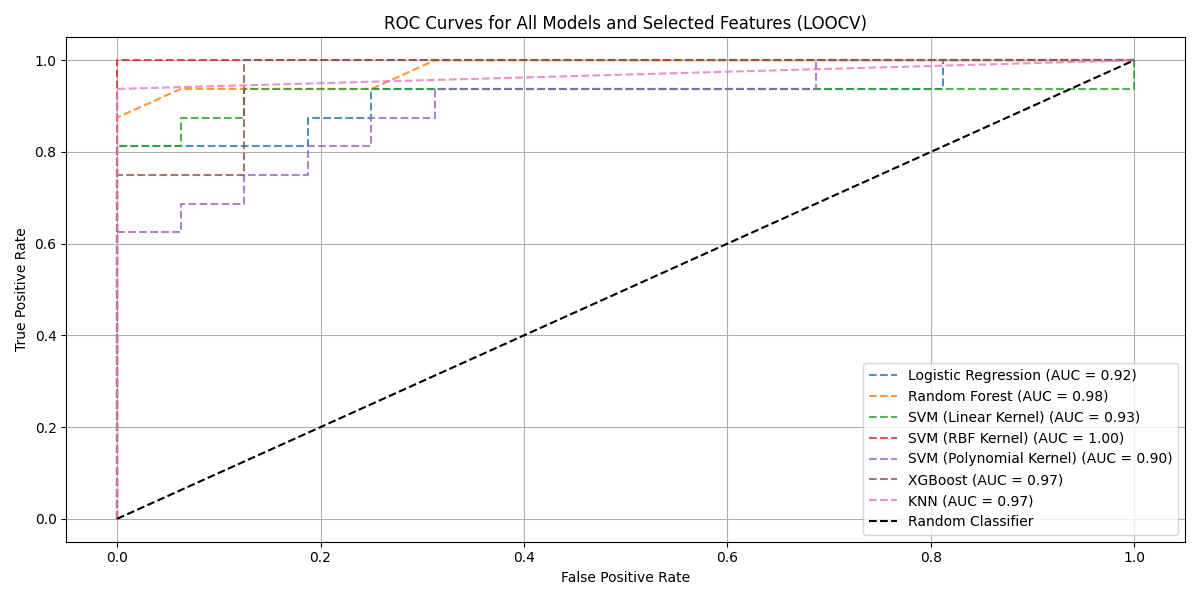
\includegraphics[width=0.5\textwidth]{Images/selected_features_models_roc_curves.png}
    \caption{ROC Curves for All Classifiers Using LOOCV}
    \label{fig:roc_curves}
\end{figure}


\subsection{Confusion Matrix Evaluation}

Fig.~\ref{fig:confusion_matrices} illustrates the confusion matrices for each classifier. Most models performed well on both classes, showing strong 
diagonal dominance. Notably, \textit{KNN}, \textit{Logistic Regression}, and \textit{SVM (Linear/RBF)} each misclassified only one instance, yielding 
very low false positive and false negative rates. In contrast, \textit{XGBoost} and \textit{Random Forest} demonstrated more balanced misclassification 
across both classes.

\begin{figure*}[htbp]
    \centering
    % Top row: 3 SVMs
    \begin{subfigure}[t]{0.30\textwidth}
        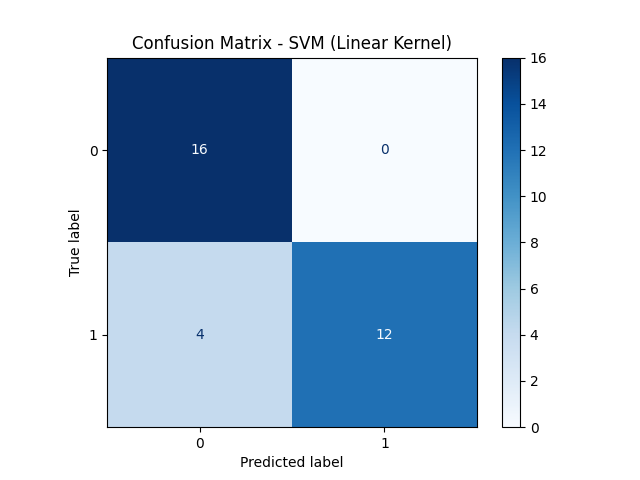
\includegraphics[width=\linewidth]{Images/confusion_matrix_svm_(linear_kernel).png}
        \caption{SVM (Linear Kernel)}
    \end{subfigure}
    \hfill
    \begin{subfigure}[t]{0.30\textwidth}
        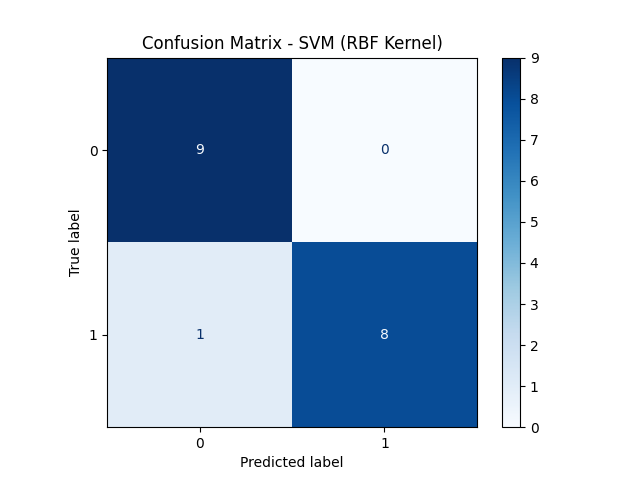
\includegraphics[width=\linewidth]{Images/confusion_matrix_svm_(rbf_kernel).png}
        \caption{SVM (RBF Kernel)}
    \end{subfigure}
    \hfill
    \begin{subfigure}[t]{0.30\textwidth}
        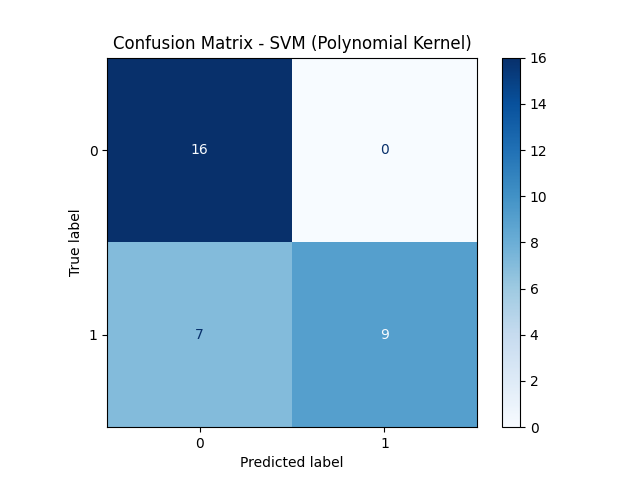
\includegraphics[width=\linewidth]{Images/confusion_matrix_svm_(polynomial_kernel).png}
        \caption{SVM (Polynomial Kernel)}
    \end{subfigure}

    \vspace{1em}

    % Middle row: KNN, XGBoost, Random Forest
    \begin{subfigure}[t]{0.30\textwidth}
        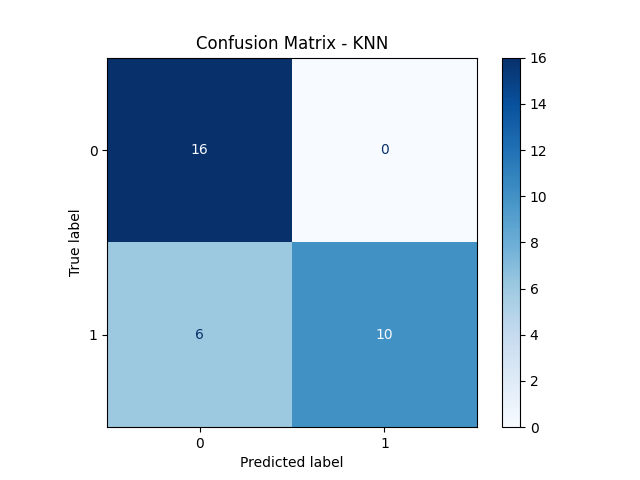
\includegraphics[width=\linewidth]{Images/confusion_matrix_knn.png}
        \caption{KNN}
    \end{subfigure}
    \hfill
    \begin{subfigure}[t]{0.30\textwidth}
        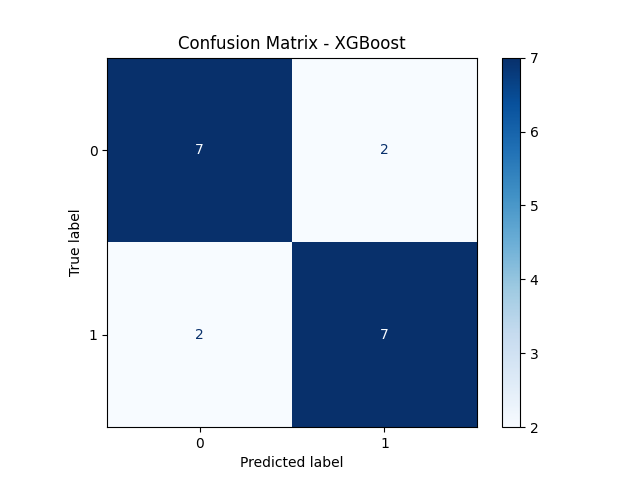
\includegraphics[width=\linewidth]{Images/confusion_matrix_xgboost.png}
        \caption{XGBoost}
    \end{subfigure}
    \hfill
    \begin{subfigure}[t]{0.30\textwidth}
        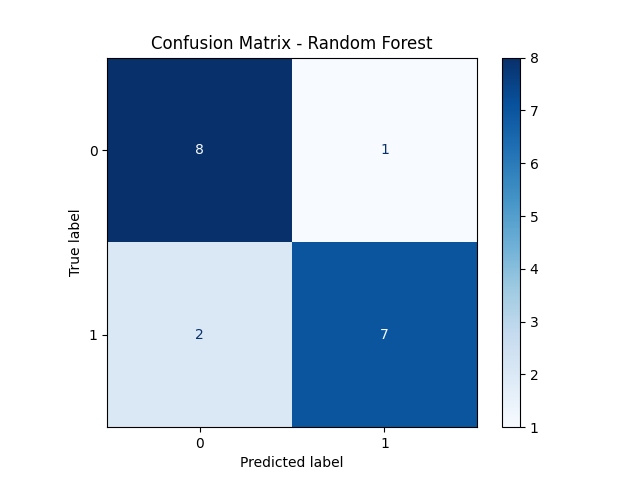
\includegraphics[width=\linewidth]{Images/confusion_matrix_random_forest.png}
        \caption{Random Forest}
    \end{subfigure}

    \vspace{1em}

    % Bottom row: Logistic Regression (centered)
    \begin{subfigure}[t]{0.30\textwidth}
        \centering
        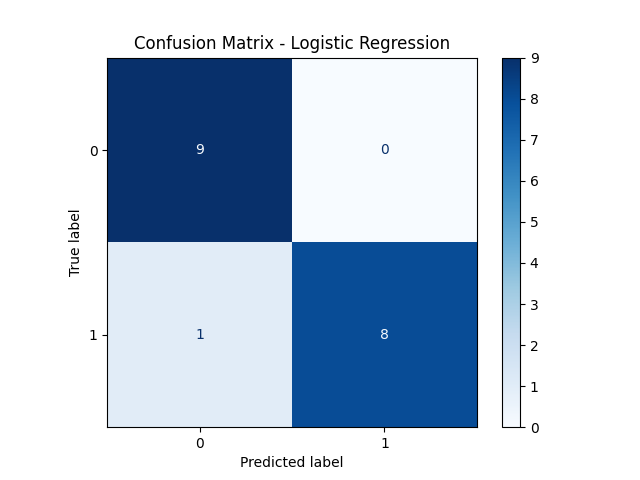
\includegraphics[width=\linewidth]{Images/confusion_matrix_logistic_regression.png}
        \caption{Logistic Regression}
    \end{subfigure}

    \caption{Confusion matrices for all classification models. Each matrix shows the number of true positive, true negative, false positive, and false negative predictions.}
    \label{fig:confusion_matrices}
\end{figure*}

\newpage
\section{Discussion}
\label{sec:discussion}

The comparative analysis of the machine learning classifiers provides insight not only into performance differences, but also into how model behavior interacts 
with the low-dimensional, subject-level feature space used in this study. Because the proposed framework relies on aggregated extremal gyroscopic features 
rather than high-frequency temporal representations, model performance is primarily governed by robustness to inter-subject variability, sensitivity to noise, 
and the ability to generalize from limited samples.

Among all models, \textit{Random Forest}, \textit{XGBoost}, and \textit{Logistic Regression} emerged as the top-performing classifiers across nearly all evaluation 
metrics. The \textit{Random Forest} model achieved the highest F1-score (93\%) and near-perfect classification in the confusion matrix, with only one instance 
misclassified. This model benefited from its ensemble learning mechanism, which combines multiple decision trees to reduce overfitting and capture complex, 
non-linear patterns in the data. Similarly, \textit{XGBoost} showed excellent generalization, with a high AUC of 0.96 and minimal misclassification, thanks to 
its gradient-boosted tree approach that optimizes classification boundaries based on prior errors. \textit{Logistic Regression}, while a linear model, also 
performed competitively (F1-score of 89\%), likely due to the high discriminative power of the selected features and the low-dimensional nature of the dataset.

In contrast, the \textit{SVMs}, especially the polynomial kernel variant, underperformed in comparison. While SVMs 
with linear and RBF kernels achieved reasonable AUC values (0.92 and 1.00 respectively), their F1-scores remained moderate (85\%), and they showed a higher 
false negative rate. This tendency to misclassify abnormal gait as normal is especially problematic in clinical applications where sensitivity to pathological cases 
is critical. The observed performance gap can be attributed to the SVMs’ sensitivity to kernel parameterization and decision boundary rigidity when operating on small, 
low-dimensional datasets, where minor variations in feature distributions can lead to suboptimal margin placement. Lastly, the \textit{KNN} model displayed the 
lowest overall performance. Its reliance on instance-based learning likely made it more susceptible to local noise and feature overlap between classes, as shown by 
its high number of misclassifications.

Compared to prior studies, the proposed approach achieves comparable or superior performance while relying on substantially fewer sensing channels and features. 
For instance, Trojaniello et al.~\cite{ref30} employed seven kinematic channels, while Pohl et al.~\cite{ref31} used both wrist and ankle IMUs to reach similar 
accuracy levels. Other works, such as those by Zhao et al.~\cite{ref28} and Li et al.~\cite{ref32}, rely on complex pipelines involving inertial navigation or 
signal decomposition, which, although effective, introduce computational and deployment overheads that limit real-world applicability.

In contrast, the proposed feature set is intentionally minimal, interpretable, and biomechanically meaningful. By focusing on extremal angular velocity values 
that directly relate to shank rotation during the gait cycle, the framework preserves discriminative power while reducing sensitivity to sensor noise, feature 
redundancy, and overfitting. These characteristics make the approach particularly suitable for embedded and wearable systems operating under computational, 
energy, and bandwidth constraints.

From an application perspective, the proposed framework is intended for screening-level detection of gait abnormalities in wearable and remote monitoring scenarios, 
where computational efficiency, robustness, and interpretability are prioritized over fine-grained severity stratification. While multi-class severity modeling 
and continuous impairment scoring are important clinical objectives, they require larger, clinically annotated datasets and were therefore considered outside the 
scope of the present study.


Although deep learning approaches such as CNN-TCNs and multilayer perceptrons~\cite{ref33,ref34} have demonstrated strong performance in gait classification, 
their reliance on large datasets and higher computational demands limits their feasibility for real-time rehabilitation and wearable deployment in small-cohort 
clinical studies. The present results demonstrate that, when feature selection is guided by biomechanical relevance and domain knowledge, classical machine 
learning models can achieve strong generalization even under constrained data conditions.

Overall, the results validate that a minimal feature set focused on medically meaningful statistics such as extremal angular velocities of the lower limbs—can 
lead to high predictive performance when paired with appropriately selected classifiers. The combination of simple IMU-derived features, lightweight modeling, 
and subject-level validation highlights a practical pathway toward deployable gait assessment tools for clinical screening and remote rehabilitation support.

\section{Conclusion and Future Work}
\label{sec:conclusion}
While this study focuses on binary classification between normal and abnormal gait, this design choice reflects the intended use of the proposed framework as a
screening-level detection tool. Binary classification enables early identification of pathological gait patterns in resource constrained wearable settings, where
computational efficiency and robustness are prioritized. Multi-class severity classification (e.g., mild, moderate, severe impairment) is currently being addressed 
in a companion study that extends the present pipeline with accelerometer data and severity aware modeling.

Provided the scope of this study a lightweight and effective machine learning framework was developed for classifying abnormal gait signals using a small number of 
clinically meaningful features derived from gyroscope data. Among the models evaluated, Random Forest, XGBoost, and Logistic Regression achieved the best overall 
performance in terms of accuracy, F1-score, and AUC, demonstrating strong generalization capabilities and low misclassification rates. In contrast, SVM-based models 
exhibited lower sensitivity, particularly in detecting abnormal gait, highlighting the importance of model selection in clinical contexts. The findings emphasize 
that even with limited features and small datasets, robust classification is achievable through proper feature engineering and algorithm choice.

Future work will focus on integrating the proposed framework into real-time gait rehabilitation systems, with on-device inference capabilities for wearable platforms. 
Additionally, we aim to extend this study by creating machine learning models that use single gait cycle data along with the current models and incorporate multi-session 
data in order to improve the robustness and adaptability of the classification system. This will enable continuous monitoring and personalized feedback for stroke patients, 
improving their rehabilitation outcomes. The ultimate goal is to develop a comprehensive gait analysis platform that can be deployed in clinical settings, providing 
healthcare professionals with real-time insights into patient progress and facilitating timely interventions.
\section{Acknowledgment}
\label{sec:acknowledgment}
The authors would like to thank the Faculty of Medicine at Prince of Songkla University for providing access to the gait dataset used in this study.
We also extend our gratitude to the clinicians and participants who contributed to the original data collection process. Special thanks to the research and 
physiotherapy teams for their support in experimental setup and data quality assurance.

This work was supported in part by the GaitRehab project, funded by the European Union. The authors also acknowledge Bioassist S.A. for its contributions 
as an external technology and research consultant during the development of the machine learning framework.

\bibliographystyle{IEEEtran}
\bibliography{references}
\begin{IEEEbiography}[{
\includegraphics[width=1in,height=1.25in,clip,keepaspectratio]{Images/a1.png}}]
    {Stamatios Orfanos} is a Ph.D. candidate in Digital Systems, University of Piraeus, Greece, where he specializes in computer vision, 
    reinforcement learning, data analysis and wearable healthcare systems. He holds a B.Sc. in Computer Science and Telecommunications and an M.Sc. 
    in Artificial Intelligence from National Research Center Demokritos and University of Piraeus. As an AI Architect and Engineer in Bioassist, he leads the 
    design and implementation of AI-driven systems, on many different fields and applications. His current research centers on developing lightweight
    machine learning algorithms for wearable sensors to support remote patient monitoring and adaptive rehabilitation.
    Mr. Orfanos is a member of IEEE and actively collaborates with clinical partners to translate his research into real-world applications.
\end{IEEEbiography}

\begin{IEEEbiography}[{
\includegraphics[width=1in,height=1.25in,clip,keepaspectratio]{Images/a2.jpg}}]
    {THANITA SANGHAN} received the B.Sc. degree in Thai traditional medicine from the Faculty of Traditional Thai Medicine, Prince of Songkla 
    University, in 2009, and the M.Sc. degree in biomedical engineering from the Faculty of Medicine, in 2012. She is currently pursuing the Ph.D.
    degree in biomedical engineering with the Faculty of Medicine, Prince of Songkla University. Her research interests include gait analysis, gait 
    biomechanics, hemiplegic gait, and stroke rehabilitation. She is also involved in a Horizon Europe: gaitREHub Project focused on developing 
    intelligent wearable system for enhanced personalized gait rehabilitation.
\end{IEEEbiography}

\begin{IEEEbiography}[{
\includegraphics[width=1in,height=1.25in,clip,keepaspectratio]{Images/a3.jpg}}]
    {SURAPONG CHATPUN} received the B.Eng. degree in mechanical engineering from Chulalongkorn University, Thailand, in 1996, and the M.Eng. 
    degree from the University of Tokyo,Japan, in 2003, and the Ph.D. degree in bioengineering from the University of California, USA,
    in 2010. He currently leads the Cardiovascular Engineering Research Laboratory (CERLab) at the Faculty of Medicine, Prince of Songkla 
    University. His research interests include applying engineering approaches, such as continuum mechanics, numerical methods (e.g.FEM), 
    fluid mechanics (e.g. CFD), image processing and computer-aided design, combined with life sciences knowledge and available technologies
    to enhance understanding of circulatory system’s function and mechanisms in both normal and pathological conditions. He also designs and invents
    medical devices not only for cardiovascular applications but also for other clinical areas, such as rehabilitation and orthopedics. He is also 
    coordinating a Horizon Europe: gaitREHub project in the field of the intelligent wearable system for enhanced personalized gait rehabilitation.
\end{IEEEbiography}

\begin{IEEEbiography}[{
\includegraphics[width=1in,height=1.25in,clip,keepaspectratio]{Images/a4.jpg}}]
    {ANDREAS MENYCHTAS} 
\end{IEEEbiography}

\begin{IEEEbiography}[{
\includegraphics[width=1in,height=1.25in,clip,keepaspectratio]{Images/a4.jpg}}]
    {CHRISTOS PANAGOPOULOS} 
\end{IEEEbiography}

\begin{IEEEbiography}[{
\includegraphics[width=1in,height=1.25in,clip,keepaspectratio]{Images/a4.jpg}}]
    {ILIAS MAGLOGIANNIS} (M'00-SM'11) re-ceived a Diploma in Electrical \& Computer Engineering and a Ph.D. in Biomedical Engineering and Medical 
    Informatics from the National Technical University of Athens (NTUA). He is now Professor and Director of the Computational Biomedicine 
    Laboratory in the Dept. of Digital Systems in the University of Piraeus. His scientific interests include Biomedical Informatics, 
    Computer Vision, AI, Multimedia Processing and Pervasive Healthcare Systems. He has been engaged as principal investigator in many European and 
    National Research programs. His published scientific work includes five (5) books and more than 400 journal and conference papers, while has 
    received more than 8200 citations on his published work. He is a senior member of the IEEE, ACM, SPIE, president of IFIP Working Group WG12.5 
    (AI Applications) and vice president of IEEE EMBS Greek chapter.
\end{IEEEbiography}

\EOD

\end{document}
